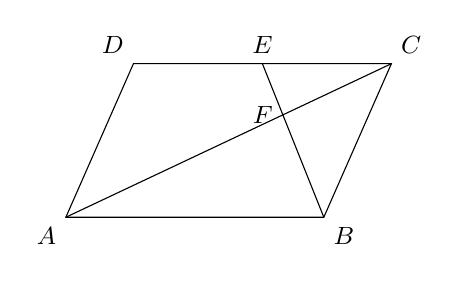
\begin{tikzpicture}[scale=.78, every node/.style={font=\small}]
  \coordinate (A) at (0,0); \coordinate (B) at (4.20,0);
  \coordinate (C) at (5.30,2.50); \coordinate (D) at (1.10,2.50);
  \coordinate (E) at (3.20,2.50); \coordinate (F) at (3.53,1.67);
  \draw (A)--(B)--(C)--(D)--cycle;
  \draw (A)--(C) (E)--(B);
  \node[below left] at (A) {$A$};
  \node[below right] at (B) {$B$};
  \node[above right] at (C) {$C$};
  \node[above left] at (D) {$D$};
  \node[above] at (E) {$E$};
  \node[left] at (F) {$F$};
\end{tikzpicture}
